\documentclass[a4paper, 12pt]{article}
%\usepackage[textwidth=16cm,textheight=24cm]{geometry}
\usepackage[a4paper,  margin=2cm]{geometry}
\usepackage{amsmath,amssymb,gensymb}
\usepackage{color}
\usepackage{graphicx}
\usepackage {wrapfig} %text to wrap around a figure
\usepackage[font=small]{caption}
\usepackage[font = small, margin = 1cm]{subcaption}
%\usepackage{caption}
% figures
\usepackage[titletoc]{appendix}
%\usepackage[toc,page]{appendix}
\usepackage{booktabs} %tables?
\usepackage{cleveref} %clever referecing use \cref{}
\crefname{appsec}{Appendix}{Appendices}
\usepackage{floatrow}
\newfloatcommand{capbtabbox}{table}[][\FBwidth]
\usepackage{listings} % typesetting code
\usepackage{multirow} %merge rows
\usepackage{array} % to left align bullets
\usepackage{enumitem} %
\usepackage{placeins}%to use \FloatBarrier command to prevent floats appearing beyond a certain point
\crefname{appsec}{Appendix}{Appendices}
\usepackage{multicol} % equations  side by side
\usepackage{hyperref} % hyperlinks
\usepackage{tikz}
\usetikzlibrary{decorations.markings}
\usepackage{pgfplots} % draw algebraic graphs
\usepackage[T1]{fontenc}
\usepackage{stix}
\usepackage{multicol}

%\newcommand{\HRule}{\rule{\linewidth}{0.1mm}} 

%\graphicspath{{C:/Users/RAK/Documents/IIB/4M20_/Report/pics/}}https://preview.overleaf.com/public/qdbmzhxkmxwb/images/606894b7399bf4cabf3b6db073a52e5bef413281.jpeg
\DeclareGraphicsExtensions{.png,.jpg,.PNG,.jpeg}

\begin{document}
\captionsetup[subfigure]{font=footnotesize}
\vspace{-1cm}
% \begin{center}
% {\LARGE{{\textbf{Analysis and Design of Relay Feedback Systems}}}}\vspace{0.1cm}\\
% { Rajiv Kurien }
% \end{center}
\title{Analysis and Design of Relay Feedback Systems}
\author{Rajiv Kurien}
\date{ }
\maketitle
\vspace{-.5cm}
%\begin{center}
%\emph{Rajiv Kurien}%
%\end{center}

% \section*{Abstract}
\abstract
\color{black}
Several models of biological oscillations consist of a cascade of linear differential equations and one non-linear differential equation. The non-linearity is often a `decision' or `on/off'. Modelling this type of non-linearity using a relay feedback system, transforms the analysis of  oscillations to classical control theory. By simplying a model into relay feedback form, the theory behind oscillations in relay feedback systems can be used to gain insight on how the model depends on different parameters. This report explores modelling biological oscillations as relay feedback systems.

\section{Introduction}
\color{black}
\subsection{Biological oscillations}
With the rapid development of computer simulations, models of biological oscillations have become increasingly complex. Large cascades of differential equations model different reactions in a pathway, but they become more difficult to understand and analyse. Furthermore, as the number of parameters increase, analysing their effect on the oscillations is difficult. 
Additionally, many oscillations in biology have a digital behaviour, such as:
\begin{enumerate}
\item Gene on/off --- negative feedback with the product of the gene. 
\item Action potential --- all or nothing principle based on whether a threshold in exceeded.
\end{enumerate}
These oscillations couple analogue and digital signals, much like oscillations in relay feedback systems. 

\subsection{Relay feedback}
A relay is a particular type of non-linear element that has only two outputs, a high or a low value, dependent on the input. Figure \ref{relay_element} shows a symmetric relay element that satisfies the input ($e$) and output ($u$) relationship:
\begin{equation}
	u(t)=\begin{cases}
	               d \text{ if } e > \epsilon \text{ or } (e >-\epsilon \text{ and } u(t-) = d)\\
	                -d \text{ if } e < -\epsilon \text{ or } (e < \epsilon \text{ and } u(t-) = -d)\\
	              
	            \end{cases}
\end{equation}


\begin{figure}[h!]
\RawFloats
\centering
\color{black}
\begin{minipage}[b]{0.25\textwidth}
 \tikzstyle arrowstyle=[scale=1]
  \tikzstyle directed=[postaction={decorate,decoration={markings,
      mark=at position .9 with {\arrow[arrowstyle]{stealth}}}, mark = at position .9 with {\arrow[arrowstyle]{stealth}}}]
  \begin{center}
  \begin{tikzpicture}[scale = 0.6]
    \draw [->, very thick] (-3,0)  node (xaxis_right){} -- (3, 0) node (xaxis_left) [below] {  $e$};
    \draw [->, very thick] (0,-3)  node (yaxis_bottom){} -- (0, 3) node (yaxis_top) [right] { $u$};
    \draw [directed, thick, blue] (3,2) node(relay_top_right){} --(-1,2) node (relay_top_left){};
    \draw[directed, thick, blue] (-3,-2) node(relay_bottom_left){}--(1,-2) node (relay_bottom_right){};
    \draw[directed, thick, blue] (-1,2) node{} -- (-1,-2) node {};
    \draw[directed, thick, blue] (1,-2) node{} -- (1,2) node {};

    \draw (1,0) node [below right]{ $\epsilon$}; %label
    \draw (-1,0) node [below left]{ $-\epsilon$}; %label
    \draw (0,2) node [above left]{ $d$}; %label
    \draw (0,-2) node [below left]{ $-d$}; %label
	\end{tikzpicture}
	\end{center}
		 \captionof{figure}{Relay element}%
		 \label{relay_element}%
	\end{minipage}%
\qquad%
	\begin{minipage}[b]{0.5\textwidth}
		\tikzstyle{block} = [draw, fill=white, rectangle, 
    minimum height=3em, minimum width=6em]
\tikzstyle{sum} = [draw, fill=white, circle, node distance=1cm]
\tikzstyle{input} = [coordinate]
\tikzstyle{output} = [coordinate]
\tikzstyle{pinstyle} = [pin edge={to-,thin,black}]

% The block diagram code is probably more verbose than necessary
\begin{center}
\resizebox{7cm}{!}{%
\begin{tikzpicture}[auto, node distance=2cm,>=latex]
    % We start by placing the blocks
    \node [input, name=input] {};
    \node [sum, right of=input] (sum) {};
    \node [block, right of=sum] (relay) {Relay};
    \node [block, right of=relay, node distance = 3.5cm] (plant) {Plant};
    % We draw an edge between the controller and system block to 
    % calculate the coordinate u. We need it to place the measurement block. 
    \draw [->] (relay) -- node[name=u] {$u$} (plant);
    \node [output, right of=plant] (output) {};
    \node [output, below of=u] (measurements) {Measurements};

    % Once the nodes are placed, connecting them is easy. 
    \draw [draw,->] (input) -- node {$r = 0$} (sum);
    \draw [->] (sum) -- node {$e$} (relay);
    \draw [->] (plant) -- node [name=y] {$y$}(output);
    \draw [-] (y) |- (measurements);
    \draw [->] (measurements) -| node[pos=0.99] {$-$} 
        node [near end] {} (sum);
\end{tikzpicture}
}
\end{center}
	\captionof{figure}{Relay feedback}
	\label{relay_feedback}
\end{minipage}
\end{figure}
\begin{figure}[h!]
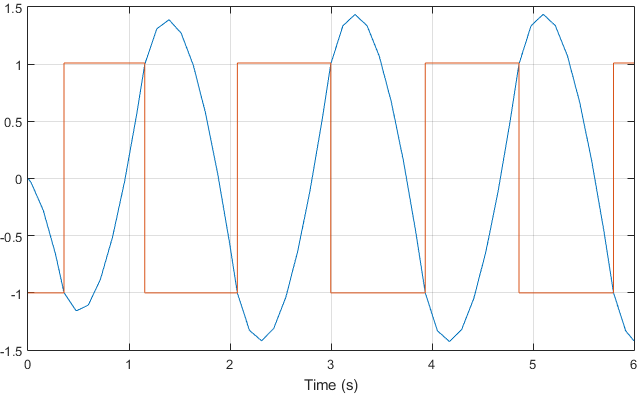
\includegraphics[height = 0.25\textwidth]{relay_feedback_oscillations}
\caption{Oscillations in a relay feedback system. The relay is orange, and plant is blue.}
\label{relay_feedback_oscillations}
\end{figure}
\color{black}
Figure \ref{relay_feedback} reveals how a typical relay feedback system is connected. The output of a plant ($y$), is connected to the relay ($e = -y$), and the output of the relay is input to the plant. Relay feedback systems tend to cause oscillations as the plant is subjected to maximal input (high or low) in the opposite direction when the plant exceeds a threshold ($\epsilon$ or $-\epsilon$), as shown in  Figure \ref{relay_feedback_oscillations}. 
\color{black}
The most popular use of relay feedback systems is for autotuning PID controllers. Automatic tuners use the oscillations to get information regarding phase margins. The relay feedback auto-tuning technique has several more attractive features\cite{hang}.
\color{black}
Relay feedback systems combine analogue and digital signals and can thus model switching behaviour in biological oscillations. Furthermore, the theory developed for analysing relay feedback systems give a tool, using which biological oscillations can be analysed. Specifically, the linear part of the biological model can be grouped together to form the plant while the non-linearity is modelled as a relay. The rest of the paper carries this out on two fundamental models of oscillations in biology: (1) FitzHugh-Nagumo model for action potentials and (2) Goodwin oscillator model for circadian rhythms. 

%\section{Theory}
The main theory used in this report is from \cite{astrom1995}. It derived for oscillations in relay feedback systems:
\begin{enumerate}
\item Conditions for oscillations
\item Initial conditions for oscillations
\item Local stability conditions
\end{enumerate}
\color{black}
\noindent Transforming models to relay feedback form allows one to analyse the effect of different parameters by using the above theory. 
\vspace{-.5cm}
\section{Modelling biological oscillations}
\subsection{FitzHugh-Nagumo model}
The FitzHugh-Nagumo model for action potentials describe the voltage-current relationship across the nerve cell membrane : \vspace{-0.5cm}
\begin{align}
\label{f_n_equations1}
\epsilon \dot{v} &= f(v) - w + I_{\text{app}}\\
\label{f_n_equations2}
\dot{w} &= v - \gamma w 
\end{align}
where:
\begin{equation}
f(v) = v(1-v)(v-\alpha), \text{\hspace{0.4cm} for }0 <\alpha<1\text{ , } \epsilon\ll 1
\end{equation}
The voltage, $v$, changes much more rapidly than the current, $w$, because $\epsilon\ll 1$. $I_{\text{app}}$ is the externally applied current (the stimulus), and it will be kept constant in order to produce continuous oscillations. $f(v)$ can be viewed as a non-linear resistor; it is the (cubic) nullcline\footnote{Nullcline of a variable $x$ is defined as where $\dot{x} = 0$} for $v$. The nullcline for $w$ is linear. With  $\alpha = 0.1, \gamma = 0.5, \epsilon = 0.01$ and $I_{\text{app}} = 0.5$, the unique rest point (where the two nullclines intersect) is unstable. This results in stable periodic oscillations \cite{keener} as reproduced in Figure \ref{fitz-nagumo}.
\color{black}
\begin{figure}[h!]
    \centering
    \begin{subfigure}[t]{0.49\textwidth}
        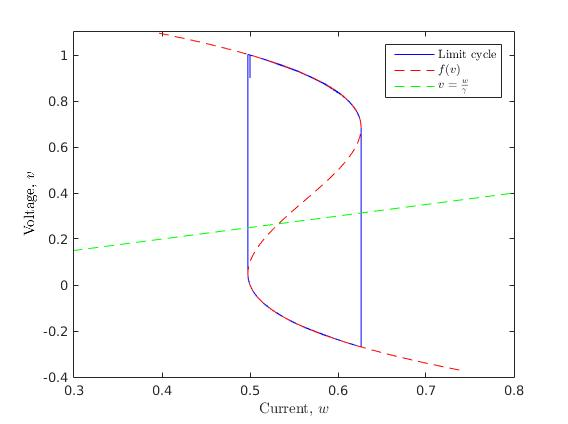
\includegraphics[width=\textwidth]{tmr_fn_limit_cycle}
        \caption{Phase Portrait. Voltage is like the output of a skewed relay. The dashed lines are nullclines (red fo voltage and green for current). }
        \label{fitz_nagumo_hysteresis}
    \end{subfigure}
     %add desired spacing between images, e. g. ~, \quad, \qquad, \hfill etc. 
    %(or a blank line to force the subfigure onto a new line)
    \begin{subfigure}[t]{0.49\textwidth}
        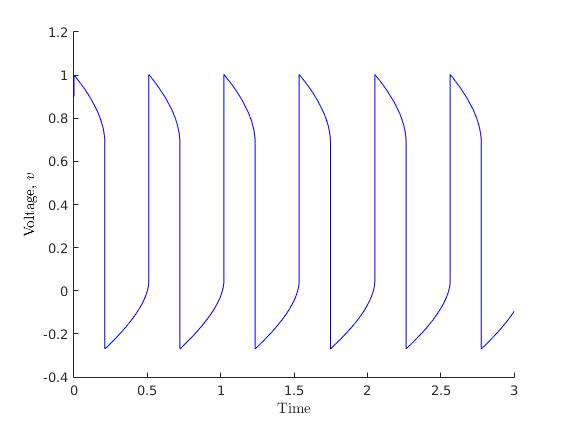
\includegraphics[width=\textwidth]{tmr_fn_voltage}
        \caption{Voltage oscillations against time. Voltage alternates between a high state and a low state.}
        \label{f_n}
    \end{subfigure}
\caption{FitzHugh-Nagumo model with unstable unique rest point, and with $\epsilon =1\text{e}-10 $.}
\label{fitz-nagumo}
\end{figure}
\color{black}
As $\epsilon\rightarrow0$, the high gain feedback causes inversion \cite{goodwin}, and the voltage behaves like the output of a skewed relay (see phase portrait Figure \ref{fitz_nagumo_hysteresis}). Using a shift in co-ordinates to make the relay symmetric around the origin and a change of basis so that an unskewed relay can be used (allowing us to use the work in \cite{astrom1995}) results in the relay feedback system in Figure \ref{fitz_nagumo_relay_block_diagram}. The details of this transformation are illustrated in the Appendix.  

\begin{figure}[h!]

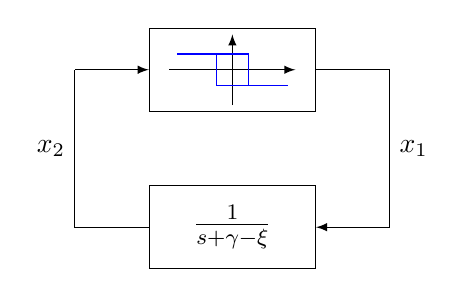
\begin{tikzpicture}[auto, node distance=2cm,>=latex, scale = 0.25]
\tikzstyle{block} = [draw,  rectangle,  minimum height=3em, minimum width=6em]
\tikzstyle{sum} = [draw,  circle, node distance=1cm]
\tikzstyle{input} = [coordinate]
\tikzstyle{output} = [coordinate]
\tikzstyle{pinstyle} = [pin edge={to-,thin,black}]   % We start by placing the blocks

\def\relay{
\tikz[remember picture,overlay]{
\draw[->] (-.8,0) -- (.8,0);
\draw[->] (0,-0.45)--(0,0.45);
\draw[blue] (0.7,-0.2)--(0.2,-0.2)--(0.2,0.2)--(-.7,.2);
\draw[blue] (-.2,.2)--(-.2,-.2)--(.2,-.2);
}}

    \node [block] (inverse) {};
    \node[] at (inverse) {\relay};
    \node [output, right of = inverse] (output) {};
    \node [input, left of = inverse](input){};
    \node [block, below of = inverse](linear_tf){\large $\frac{1}{s+\gamma-\xi}$};

    % Once the nodes are placed, connecting them is easy. 
    \draw [-] (inverse) -- (output);
    \draw [->] (output) |- node[near start] {$x_1$}(linear_tf);
    \draw [-] (linear_tf) -| node[near end] {$x_2$} (input);
    \draw [->] (input) -- (inverse);

\end{tikzpicture}
\caption{Relay feedback model of FitzHugh-Nagumo.}
\label{fitz_nagumo_relay_block_diagram}
\end{figure}
\color{black}
For this relay feedback system, \cite{astrom1995} predicts oscillations of a time period, $T=2h$, such that: 
\begin{equation}
C\left(I + e^{Ah}\right)^{-1} \int_0^h e^{As}Bds = \frac{\epsilon}{d} 
 \end{equation}
For this system, only one solution exists which shows the existence of one limit cycle, with time period of 0.543 seconds. Furthermore, it was shown to be locally stable. The simulation shown in Figure \ref{matching_fitz_relay} does indeed have the predicted time period and the oscillations matches the FitzHugh-Nagumo model's oscillations as $\epsilon\rightarrow0$. 

This example reveals how classical control theory of relay feedback systems is able to give analytical results for particular oscillatory models. This bridging of biological models with relay feedback gives tools which can be used as a first step in analysing the effect of different parameters on existence of limit cycles, local stability, time periods. 

\begin{figure}[h!]
    \centering
    \begin{subfigure}[t]{0.45\textwidth}
        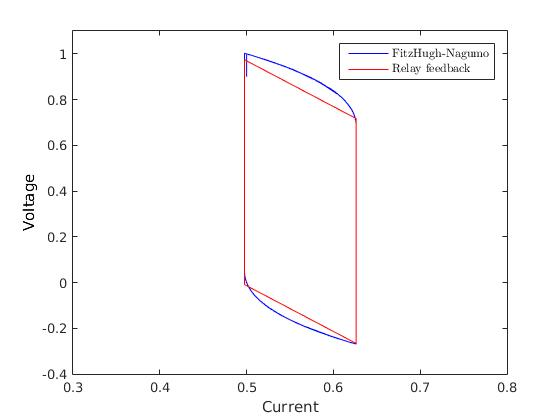
\includegraphics[width=\textwidth]{tmr_fn_relay_limit_cycle}
        \caption{Phase Portrait. Voltage is like the output of a skewed relay.}
        \label{f_n_relay_limit_cycle}
    \end{subfigure}
    ~ %add desired spacing between images, e. g. ~, \quad, \qquad, \hfill etc. 
    %(or a blank line to force the subfigure onto a new line)
    \begin{subfigure}[t]{0.45\textwidth}
        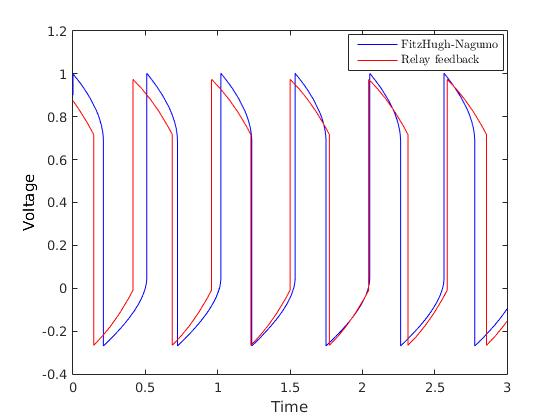
\includegraphics[width=\textwidth]{tmr_fn_relay_voltage}
        \caption{Voltage oscillations against time. Voltage alternates between a high state and a low state.}
        \label{f_n_relay_voltage}
    \end{subfigure}
\caption{FitzHugh-Nagumo model and Relay feedback model match in $\lim\limits_{\epsilon\to 0}$}
\label{matching_fitz_relay}
\end{figure}
\FloatBarrier\vspace{-2cm}
\subsection{Goodwin oscillator}

The Goodwin oscillator is a biochemical oscillator based on negative feedback alone. It describes the mechanism of how mRNA, protein and end product interact. Written in their non-dimensional form \cite{fall}, the Goodwin oscillator's kinetic equations are:
\begin{align}
\frac{dx_1}{dt'} &= \frac{1}{1 + x_3^p} - b_1x_1 \\
\frac{dx_2}{dt'} &= b_2(x_1 - x_2) \\
\frac{dx_3}{dt'} &= b_3(x_2 - x_3)
\end{align}

\noindent The only nonlinearity, $(\frac{1}{1 + x_3^p})$, becomes a relay with no hysteresis as $p \rightarrow \infty$ (see Figure \ref{goodwin_nonlinearity}).

\begin{figure}[h!]
\RawFloats
\centering
\begin{minipage}[t]{.4\textwidth}
\centering
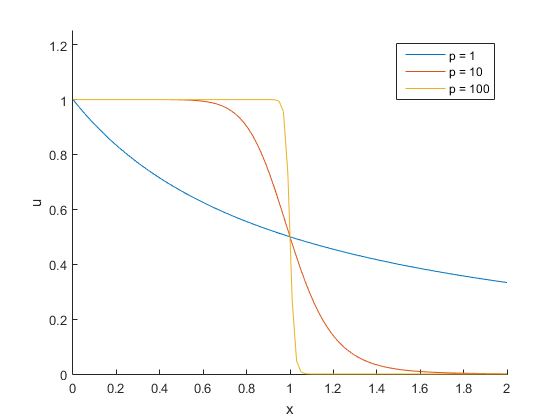
\includegraphics[width = \textwidth]{goodwin_nonlinear_element}
\caption{Nonlinearity becomes a relay with no hysteresis, as $p \rightarrow \infty$.}
\label{goodwin_nonlinearity}
\end{minipage}
\hspace{0.5cm}
\begin{minipage}[t]{0.4\textwidth}
\centering
\resizebox{6cm}{!}{%
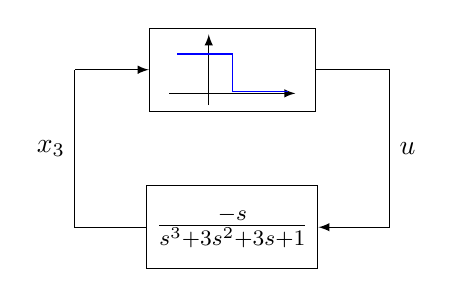
\begin{tikzpicture}[auto, node distance=2cm,>=latex]
\tikzstyle{block} = [draw,  rectangle,  minimum height=3em, minimum width=6em]
\tikzstyle{sum} = [draw,  circle, node distance=1cm]
\tikzstyle{input} = [coordinate]
\tikzstyle{output} = [coordinate]
\tikzstyle{pinstyle} = [pin edge={to-,thin,black}]   % We start by placing the blocks

\def\relay{
\tikz[remember picture,overlay]{
\draw[->] (-.8,-.3) -- (.8,-0.3);
\draw[->] (-.3,-0.45)--(-.30,0.45);
\draw[blue] (0.7,-0.28)--(0.,-0.28)--(0,0.2)--(-.7,.2);
%\draw[blue] (-.2,.2)--(-.2,-.2)--(.2,-.2);
}}

    \node [block] (inverse) {};
    \node[] at (inverse) {\relay};
    \node [output, right of = inverse] (output) {};
    \node [input, left of = inverse](input){};
    \node [block, below of = inverse](linear_tf){\large $\frac{-s}{s^3 + 3s^2 + 3s + 1}$};

    % Once the nodes are placed, connecting them is easy. 
    \draw [-] (inverse) -- (output);
    \draw [->] (output) |- node[near start] {$u$}(linear_tf);
    \draw [-] (linear_tf) -| node[near end] {$x_3$} (input);
    \draw [->] (input) -- (inverse);

\end{tikzpicture}
}
\caption{Relay feedback system model of Goodwin oscillator ($b_1=b_2=b_3=1$). }
\label{goodwin_transfer}
\end{minipage}
\end{figure}

Rewriting the equations such that the linear equations form the plant and the nonlinearity is a relay, results in the system in Figure \ref{goodwin_transfer}. 

Using the theory in \cite{astrom1995}, initial conditions for oscillations were used to initialise both models. Furthermore, these oscillations were shown to be locally stable. The simulation results, shown in Figure \ref{matching_goodwin_relay}, reveal a good match between the two models. 

\begin{figure}[h!]
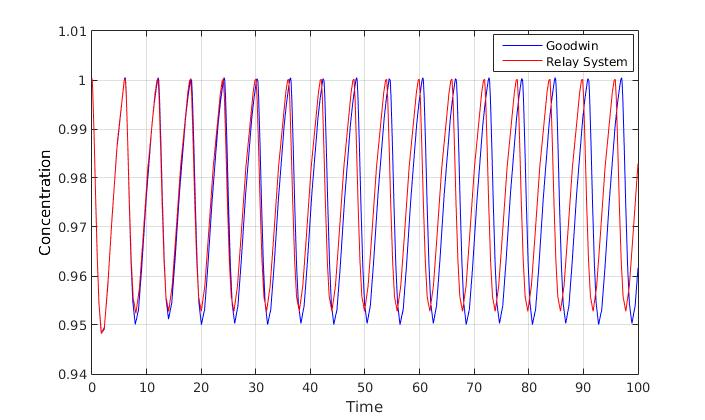
\includegraphics[width = 0.5\textwidth]{goodwin_mathcing.jpg}
\caption{Relay system models Goodwin oscillator well as $p \rightarrow \infty$.}
\label{matching_goodwin_relay}
\end{figure}

\vspace{-1cm}
\section{Future work}
Bursting is the phenomenon of rapid action potentials spiking for a period of time and then followed by a period of no activity. It features a system  with two feedback loops, which use a sigmoidal and \emph{bump} nonlinearities respectively \cite{franci}. Approximating these nonlinearities as on/off functions yields a system similar to a relay feedback, with an extra feedback loop. The next step in this project is to model a bursting circuit using relay feedback with an extra loop, and analyse this system using the approach taken in \cite{astrom1995} to derive conditions for oscillations.

\section{Conclusions}
Relay feedback was used to model two fundamental oscillations in biology. The theory behind relay feedback oscilations gave tools using which existence of limit cycles could be tested, their time period, initial conditions and local stability. This reveals the potential for certain complex biological oscillations to be simplified into the relay feedback form in order to gain insights on conditions for oscillations and stability. Future work will involve extending the same principles of simplifying oscillations using on-off non-linearities to that of bursting models. The aim is to get analytical conditions for oscillations in bursting models, expanding the potential of relay feedback systems to analyse oscillations.  


%\begin{multicols}{1}
\begin{thebibliography}{9}

\bibitem{goldbeter} A.Goldbeter, (1995) \emph{A model for circadian oscillations in the Drosophila period protein (PER)}. Proc. R. Soc. Lond. B. Volume 261, Pages 319-324. 

\bibitem{hang} C.C.Hang, K.J.\r{A}str\"{o}m, Q.G.Wang, (2002) \emph{Relay feedback auto-tuning of process controllers --- a tutorial review.} Journal of Process Control, Volume 12, Pages 143-162. 

\bibitem{astrom1995}
K.J.\r{A}str\"{o}m , (1995) \emph{Oscillations in systems with relay feedback}. IMA Vol. Math. Appl. : Adap. Control, Filtering, Signal Processing, Volume 74, Pages 1-25. 

\bibitem{keener}
J.Keener and J.Sneyd, \emph{Mathematical Physiology}. Springer-Verlag New York. Volume 8/I. Second Edition. ISBN 978-0-387-75846-6. 

\bibitem{goodwin}G.C.Goodwin, S.F.Graebe, M.E.Salgado, (2000). \emph{Control System Design}. Prentice Hall, ISBN 978-0-13-958653-8.

\bibitem{fall}
C.P.Fall, E.S.Marland, J.M.Wagner, J.J.Tyson, \emph{Computational Cell Biology}. Springer. Volume 20. ISBN 0-387-95369-8. 

\bibitem{franci}
A.Franci and R.Sepulchre, (2014). \emph{Realization of nonlinear behaviours from organizing centers.} Proc. 53st. IEEE Conf. Decision Contr., Pages 56-61.

\end{thebibliography}
%\end{multicols}

\newpage
\begin{appendices}
\appendixpage
\crefalias{section}{appsec}
\renewcommand{\thefigure}{A\arabic{figure}}
\setcounter{figure}{0}
\label{Appendix}
\section{FitzHugh-Nagumo to standard relay feedback}\vspace{-.8cm}

\begin{figure}[h!]
\begin{subfigure}[t]{.4\textwidth}

\centering
\tikzstyle{block} = [draw,  rectangle,  minimum height=3em, minimum width=6em]
\tikzstyle{sum} = [draw,  circle, node distance=1cm]
\tikzstyle{input} = [coordinate]
\tikzstyle{output} = [coordinate]
\tikzstyle{pinstyle} = [pin edge={to-,thin,black}]
\resizebox{5cm}{!}{%
  % The block diagram code is probably more verbose than necessary
  \begin{tikzpicture}[auto, node distance=2cm,>=latex,scale=0.75]
      % We start by placing the blocks
      \node at (0,3) (I_app) {$I_{app}$};
      %\node[input, name = I_app]{text};
      \node[sum, right of = I_app](sum_outer){};
      \node [sum, right of = sum_outer] (sum_inner) {};
      \node [block, right of = sum_outer, node distance=3cm] (high_gain) {\large{$\frac{1}{\epsilon s}$}};
      % We draw an edge between the controller and system block to 
      % calculate the coordinate u. We need it to place the measurement block. 
      \node [output, right of = high_gain] (output) {};
      \node [block, below of = high_gain] (cubic_nullcline) {$f(\cdot)$};
      \node [block, below of = cubic_nullcline](linear_tf){\large $\frac{1}{s+\gamma}$};

      % Once the nodes are placed, connecting them is easy. 

      % inner loop
      \draw [draw,->] (sum_outer) -- node {$+$} (sum_inner);
      \draw [->] (sum_inner) -- node {$\dot{v}$} (high_gain);
      \draw [->] (high_gain) -- node [name=v] {$v$}(output);
      \draw [->] (v) |- (cubic_nullcline);
      \draw [->] (cubic_nullcline) -| node[pos=.85] {$+$} 
          node [near end] {} (sum_inner);

      % outer loop
      \draw [->](v) |- (linear_tf);
      \draw [->](linear_tf) -| node[anchor=south,pos=0.2] {$w$} 
          node[pos=0.93]{-}(sum_outer);
      \draw [->](I_app)-- node[near end]{$+$} (sum_outer);
  \end{tikzpicture}}
	\caption{Block diagram}%
	\label{fitz_nagumo_block_diagram}%
\end{subfigure}
\hspace{0.5cm}%
\begin{subfigure}[t]{.45\textwidth}
\centering
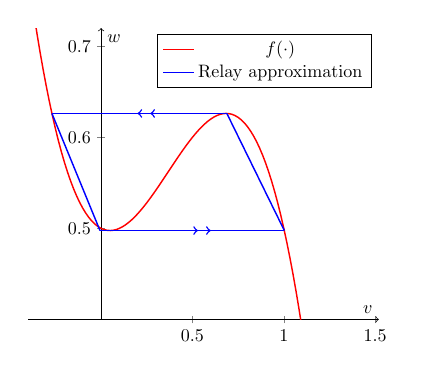
\begin{tikzpicture}[scale = 0.65]
  \begin{axis}[
    xmin=-.4,xmax=1.52,
    ymin=0.4,ymax=.72,
    axis lines=center,
    axis line style=->,
    xlabel={$v$},
    ylabel={$w$}
    ]
      \addplot[-] [color=red, style = thick] expression[domain=-0.45:1.2,samples=100]{-x^(3)+(1+0.1)*x^(2) - 0.1*x + 0.5}; 
      \addplot[-] [color=blue, style = thick] coordinates{(-.2693,0.6262) (.6883,.6262)};
            \addplot[<-] [color=blue, style = thick] coordinates{(.2693,0.6262) (.6883,.6262)};
            \addplot[<-] [color=blue, style = thick] coordinates{(.1993,0.6262) (.6883,.6262)};
      \addplot [color=blue, style = thick] coordinates{(.6883,0.6262) (1.003,.4976)};
      \addplot [color=blue, style = thick] coordinates{(-.2693,0.6262) (-.0061,.4976)};
      \addplot [-][color=blue, style = thick] coordinates{(-.0061,.4976) (1.003,.4976)};
      		\addplot [->][color=blue, style = thick] coordinates{(-.0061,.4976) (.6,.4976)};
            \addplot [->][color=blue, style = thick] coordinates{(-.0061,.4976) (.53,.4976)};
     % \addplot[-] [color=green, style = thick] expression[domain=-0.45:1.2,samples=100]{-y^(3)+(1+0.1)*y^(2) - 0.1*y + 0.5}; 
     \addlegendentry{$f(\cdot)$}
	 \addlegendentry{Relay approximation}
	\end{axis}
\end{tikzpicture}
	\caption{Nonlinearity and the ``relay" approximation}%
	\label{original_nonlinearity}%
\end{subfigure}
\caption{FitzHugh-Nagumo}
\label{fn}
\end{figure}

\vspace*{-.5cm}

\begin{figure}[h!]
\RawFloats
\centering
\begin{minipage}[t]{.45\textwidth}
\centering
\tikzstyle{block} = [draw,  rectangle,  minimum height=3em, minimum width=6em]
\tikzstyle{sum} = [draw,  circle, node distance=1cm]
\tikzstyle{input} = [coordinate]
\tikzstyle{output} = [coordinate]
\tikzstyle{pinstyle} = [pin edge={to-,thin,black}]

% The block diagram code is probably more verbose than necessary
\resizebox{4cm}{!}{%
\begin{tikzpicture}[auto, node distance=2cm,>=latex, scale = 0.5]
    % We start by placing the blocks
    \node at (0,3) (I_app) {$I_{app}$};
    %\node[input, name = I_app]{text};
    \node[sum, right of = I_app](sum_outer){};
    \node [block, right of = sum_outer] (inverse) {$-f^{-1}(\cdot)$};
    \node [output, right of = inverse] (output) {};
    \node [block, below of = inverse](linear_tf){\large $\frac{1}{s+\gamma}$};

    % Once the nodes are placed, connecting them is easy. 
    \draw [->] (sum_outer) --(inverse);
    \draw [->] (inverse) -- node [name=v] {$v$}(output);
    \draw [->](v) |- (linear_tf);
    \draw [->](linear_tf) -| node[anchor=south,pos=0.2] {$w$} 
    	node[pos=0.93]{-}(sum_outer);
    \draw [->](I_app)-- node[near end]{$+$} (sum_outer);
\end{tikzpicture}
}
	\captionof{figure}{High gain inversion}%
	\label{high_gain_inversion}%
\end{minipage}
\hspace{.5cm}
\begin{minipage}[t]{.45\textwidth}
\centering
\tikzstyle{block} = [draw,  rectangle,  minimum height=3em, minimum width=6em]
\tikzstyle{sum} = [draw,  circle, node distance=1cm]
\tikzstyle{input} = [coordinate]
\tikzstyle{output} = [coordinate]
\tikzstyle{pinstyle} = [pin edge={to-,thin,black}]
% The block diagram code is probably more verbose than necessary
\resizebox{4cm}{!}{%
\begin{tikzpicture}[auto, node distance=2cm,>=latex]
    % We start by placing the blocks
    \node at (0,3) (I_app) {$I_{app}$};
    %\node[input, name = I_app]{text};
    \node[sum, right of = I_app](sum_outer){};
    \node [block, right of = sum_outer] (inverse) {$f_{2}(\cdot)$};
    \node [output, right of = inverse] (output) {};
    \node [block, below of = inverse](linear_tf){\large $\frac{1}{s+\gamma}$};

    % Once the nodes are placed, connecting them is easy. 
    \draw [->] (sum_outer) --(inverse);
    \draw [->] (inverse) -- node [name=v] {$v$}(output);
    \draw [->](v) |- (linear_tf);
    \draw [->](linear_tf) -| node[anchor=south,pos=0.2] {$w$} 
    	node[pos=0.93]{+}(sum_outer);
    \draw [->](I_app)-- node[near end]{$-$} (sum_outer);
\end{tikzpicture}
}
      \captionof{figure}{$f_2(x) = -f^{-1}(-x)$}%
      \label{invert_y_axis}%
\end{minipage}
\end{figure}

\vspace{-1cm}

\begin{figure}[h!]
\begin{subfigure}[t]{0.45\textwidth}
\centering
\tikzstyle{block} = [draw,  rectangle,  minimum height=3em, minimum width=6em]
\tikzstyle{sum} = [draw,  circle, node distance=1cm]
\tikzstyle{input} = [coordinate]
\tikzstyle{output} = [coordinate]
\tikzstyle{pinstyle} = [pin edge={to-,thin,black}]

% The block diagram code is probably more verbose than necessary
\resizebox{4cm}{!}{%
\begin{tikzpicture}[auto, node distance=2cm,>=latex]
    % We start by placing the blocks
	
    \node [block] (inverse) {$f_3(\cdot)$};
    \node [output, right of = inverse] (output) {};
    \node [input, left of = inverse](input){};
    \node [block, below of = inverse](linear_tf){\large $\frac{1}{s+\gamma}$};

    % Once the nodes are placed, connecting them is easy. 
    \draw [-] (inverse) -- (output);
    \draw [->] (output) |- node[near start] {$\hat{v}$}(linear_tf);
    \draw [-] (linear_tf) -| node[near end] {$\hat{w}$} (input);
    \draw [->] (input) -- (inverse);

\end{tikzpicture}
}
\caption{Block diagram}
\end{subfigure}
\quad%
\begin{subfigure}[t]{.45\textwidth}
\centering
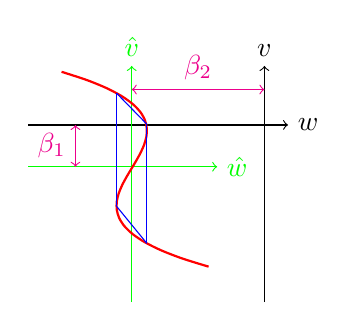
\begin{tikzpicture}[xscale=3,yscale=1.5]
  \newcommand\myscale{1};
  \draw[->] (-1*\myscale,0) -- (0.1*\myscale,0) node[right] {$w$};
  \draw[->] (0,-1.5*\myscale*\myscale) -- (0,.5*\myscale*\myscale) node[above] {$v$};
    \draw[->] [green](-1*\myscale,-.354) -- (-.2*\myscale,-.354) node[right] {$\hat{w}$};
  	\draw[->] [green](-.5619,-1.5*\myscale*\myscale) -- (-.5619,.5*\myscale*\myscale) node[above] {$\hat{v}$};
    \draw[<->][magenta](-.5619,.3) -- node[above]{$\beta_2$} (0,.3);
    \draw[<->][magenta](-.8,-.354) -- node[left]{$\beta_1$} (-.8,0);

% code for Mirror Image
\begin{scope}[xscale = -1,xshift=0cm]
  \begin{scope}[yscale=-1,yshift=0cm]
    \draw[scale=\myscale,domain=-.45:1.2,smooth,variable=\y,red, thick]  plot ({-(\y)^(3)+(1+0.1)*(\y)^(2) - 0.1*(\y) + 0.5},{\y});
    \draw[-,scale=\myscale,blue] (0.6262,-.2693) -- (0.6262,.6883);
    \draw[-,scale=\myscale,blue] (0.6262,.6883) -- (.4976,1.003);
    \draw[-,scale=\myscale,blue] (0.6262,-.2693) -- (.4976,-.0061);
    \draw[-,scale=\myscale,blue] (.4976,-.0061) -- (.4976,1.003);
  \end{scope}
  \end{scope}
\end{tikzpicture}
\caption{Nonlinearity in new co-ordinates, $f_3(\cdot)$}
\end{subfigure}
      \caption{Shift co-ordinate system to make relay symmetric, $I_{app}$ disappears. $\hat{w} = w + \beta_2$ and $\hat{v} = v + \beta_1$}%
      \label{shift1}%
\end{figure}\nopagebreak%
\begin{figure}[h!]
\RawFloats
\centering
\begin{minipage}[t]{.4\textwidth}
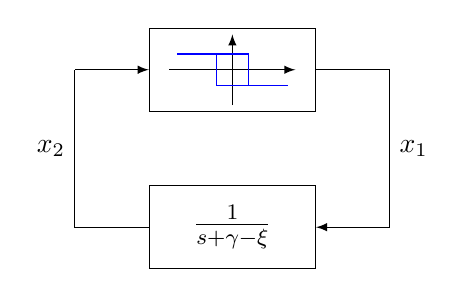
\begin{tikzpicture}[auto, node distance=2cm,>=latex]
\tikzstyle{block} = [draw,  rectangle,  minimum height=3em, minimum width=6em]
\tikzstyle{sum} = [draw,  circle, node distance=1cm]
\tikzstyle{input} = [coordinate]
\tikzstyle{output} = [coordinate]
\tikzstyle{pinstyle} = [pin edge={to-,thin,black}]   % We start by placing the blocks

\def\relay{
\tikz[remember picture,overlay]{
\draw[->] (-.8,0) -- (.8,0);
\draw[->] (0,-0.45)--(0,0.45);
\draw[blue] (0.7,-0.2)--(0.2,-0.2)--(0.2,0.2)--(-.7,.2);
\draw[blue] (-.2,.2)--(-.2,-.2)--(.2,-.2);
}}

    \node [block] (inverse) {};
    \node[] at (inverse) {\relay};
    \node [output, right of = inverse] (output) {};
    \node [input, left of = inverse](input){};
    \node [block, below of = inverse](linear_tf){\large $\frac{1}{s+\gamma-\xi}$};

    % Once the nodes are placed, connecting them is easy. 
    \draw [-] (inverse) -- (output);
    \draw [->] (output) |- node[near start] {$x_1$}(linear_tf);
    \draw [-] (linear_tf) -| node[near end] {$x_2$} (input);
    \draw [->] (input) -- (inverse);

\end{tikzpicture}
\captionof{figure}{Change of basis to use relay. $\hat{w}=x_2$ and $\hat{v} = \xi x_2 + x_1$}
\label{fn_final_block}
\end{minipage}
\hspace{0.5cm}
\begin{minipage}[t]{.4\textwidth}\vspace{-2cm}\small
Following the steps from the Figures \ref{fn} to \ref{fn_final_block} allow the standard relay to be used to model the FitzHugh-Nagumo equations. The original variables can be recovered as: 
\begin{equation*}
\begin{cases}
v = \hat{v}-\beta_1 = \xi x_2 + x_1 - \beta_1 \\
w = \hat{w}-\beta_2 = x_2 - \beta_2 \\
\end{cases}
\end{equation*}
\end{minipage}
\end{figure}


\end{appendices}
\end{document}


\end{document}